% little trick to replace lib.tex by this
\renewcommand{\doctitle}[1]{
	\chapter{#1}
}
\renewcommand{\biblio}[1]{}
\doctitle{L'oscillateur contrôlé en tension (VCO)}
\subsection{Fonctionnement et théorie}
La figure 1 nous montre le schéma bloc du VCO.
                                                                                                                                                                   

Le VCO se compose des 3 blocs suivants:
\begin{itemize}
\item l'integrator controller (le contrôleur de l'intégrateur) qui se compose lui-même d'un switch et d'un summing (sommateur)
\item l'integrator (intégrateur)
\item le trigger de Schmitt (bascule à hystérèse)
\end{itemize}

Le signal d'entrée ($in$) est constant et vaut $\alpha$. Appelons $V_L$ la tension de basculement inférieure du trigger, $V_H$ la tension de basculement supérieure et $V_{CC}$ la tension d'alimentation du trigger.
Si la sortie du trigger de Schmitt ($control$) vaut $0$, la sortie du switch de l'integrator controller vaut $0$. Dès lors, la sortie du bloc integrator controller vaut $-\alpha$.  Après passage dans l'integrator, nous avons la droite $-\alpha t$. La sortie du trigger restera à $0$ tant que la sortie de l'integrator est supérieure à $V_L$. Lorsque la sortie de l'integrator a atteint $V_L$, le trigger bascule et sa tension de sortie devient $V_{CC}$. Le switch change d'état et sa sortie devient $\alpha$. La sortie de l'integrator controller devient donc $\alpha$. Après passage dans l'integrator, nous avons la droite $\alpha t$. La sortie du trigger restera à $V_{CC}$ tant que la sortie de l'integrator est inférieure à $V_H$. Lorsque la sortie de l'integrator a atteint $V_H$, le trigger bascule et sa tension de sortie devient $0$. Le switch rechange d'état et sa sortie devient $0$. Et nous pouvons recommencer la même boucle temporelle.

\subsection{Dimensionnement et circuit réel}
\paragraph{Circuit réel}
%image circuit
Sur la figure \ref{fig:circuit_vco} se trouve l'implémentation électronique du VCO décrit ci-dessus.
\begin{figure}[ht]
\centering
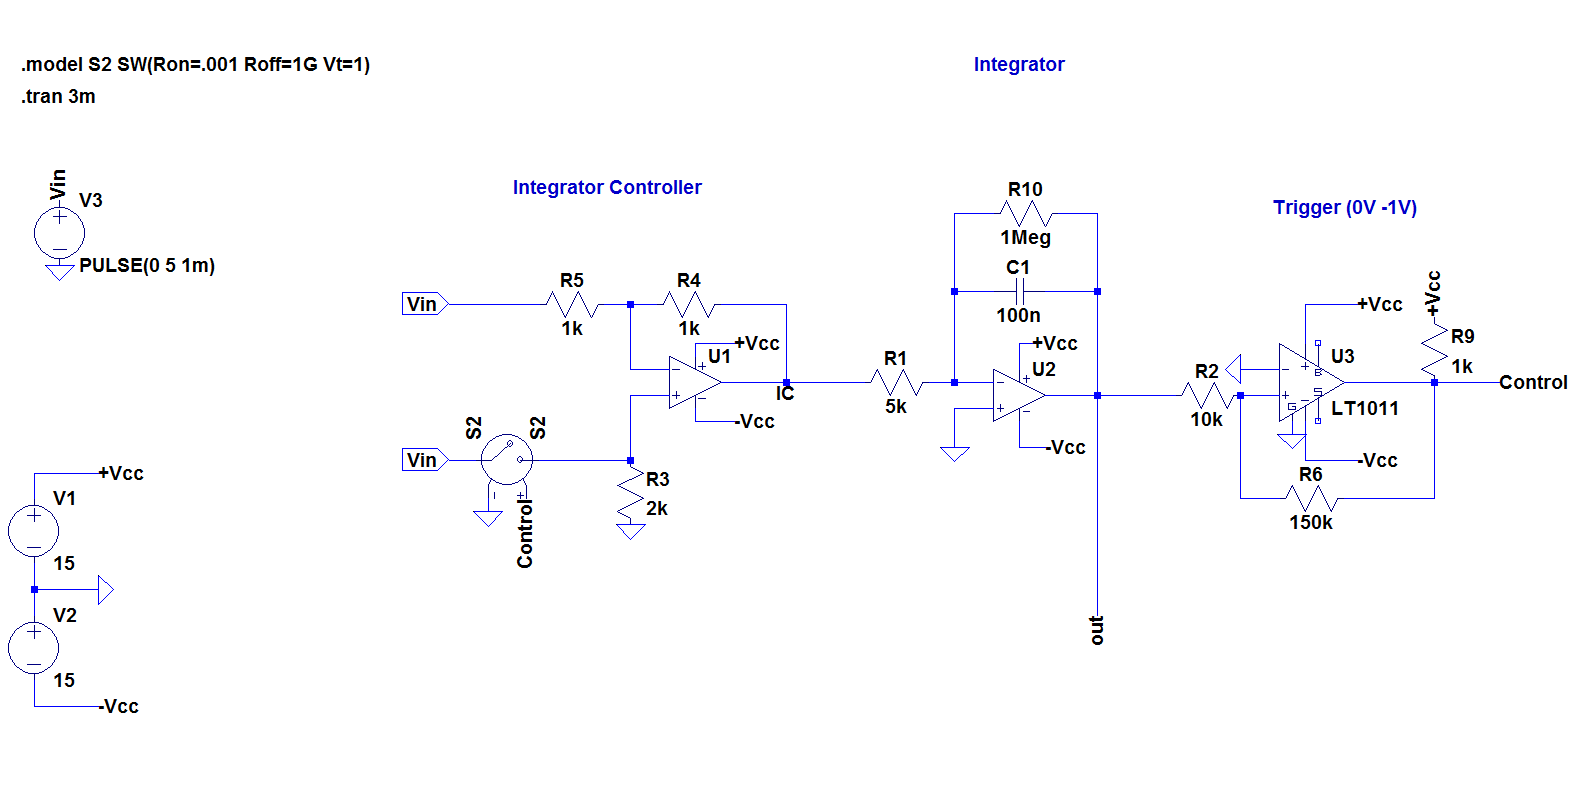
\includegraphics[width=16cm]{img/vco_circuit}
\caption{Circuit du VCO}
\label{fig:circuit_vco}
\end{figure}
\paragraph{Dimensionnement du trigger de Schmitt}
Le choix de placer le seuil supérieure ($V_H$) à \unit{0}{\volt} et le seuil inférieure ($V_L$) à \unit{-1}{\volt} est arbitraire. Cependant la différence entre $V_H$ et $V_L$ doit rester au-dessus de \unit{500}{\milli\volt} pour éviter une influence des tensions parasites. Dans ce circuit, un trigger asymétrique est utilisé. Dès lors, le rapport des résistances à utiliser se déduit des formules suivantes : 
$$V_H=V_{REF}\left(1+\frac{R_2}{R_6}\right) \textmd{ et } V_L=V_{REF} + \frac{R_2}{R_6}\left(V_{REF}-V_{CC}\right)$$
Dans le montage du trigger asymétrique utilisé, $V_{REF}$, la tension à l'entrée non-inverseuse du comparateur vaut \unit{0}{\volt}. Dès lors, $\frac{R_2}{R_6}=\frac{1}{15}$
avec la condition que $R_6>>R_9$. Les valeurs de résistances choisies sont :
\begin{itemize}
\item \unit{10}{\kilo\ohm} pour $R_2$
\item \unit{150}{\kilo\ohm} pour $R_6$.
\end{itemize}

\paragraph{Dimensionnement de l'integrator}
Calculons maintenant la constante ($K$) du bloc integrator. Le VCO doit satisfaire la relation tension fréquence suivante : \unit{1}{\milli\volt} par \unit{}{\hertz}. Si la tension d'entrée est de \unit{1}{\milli\volt}, la fréquence de sortie est de \unit{1}{\hertz}. Comme le signal de sortie est un signal triangulaire, le temps de montée et de descente est identique. Le temps de montée vaut donc $\frac{1}{2*1} =  \unit{0,5}{\second}$. La pente de montée de la droite est de \unit{1}{\milli\volt}/\unit{}{\second}. Le temps pour monter ou descendre de \unit{1}{\volt} est de \unit{1000}{\second}. Comme il doit valoir \unit{0,5}{\second}, la constante d'intégration vaut 2000. D'où $\frac{1}{R_1C_1}=2000$ avec $C_1= \unit{100}{\nano\farad}$, $R_1 = \unit{5}{\kilo\ohm}$.
\paragraph{Dimensionnement de l'integrator controller}
L'integrator controller est constitué d'un ampli op en mode différentiel et d'un switch. L'équation constitutive de ce bloc est : $V_{IC}=2*V_+ - V_-$ avec $V_+$ la tension à l'entrée non-inverseuse et $V_-$, la tension à l'entrée inverseuse. La formules suivantes permettant de déterminer une relation entre les résistances est obtenues en appliquant KCL : $$V_{IC}=V_+ \left(\frac{\left(R_4 + R_5\right)R_3}{R_3.R_5}\right)-V_-\left(\frac{R_4}{R_5}\right)$$ Cela nous donne donc $R_5 = R_4 = 2*R_3$.
Fixons $R_5$ à \unit{1}{\kilo\ohm}. Alors $R_4$ vaut \unit{1}{\kilo\ohm} et $R_3$ qui vaut \unit{2}{\kilo\ohm}.

\subsection{Confrontation  des mesures et de la théorie}
%TODO
\begin{figure}[ht]
	\centering
	\includegraphics[width=0.8\textwidth]{img/reponse_vco.png}
	\caption{Signaux de sortie des différents blocs}
	\label{fig:out_vco_th}
\end{figure}
Sur la figure \ref{fig:out_vco_th} se trouve les signaux aux sorties des trois blocs fonctionnels pour une tension d'entrée de \unit{5}{\volt}. En rouge, le signal à la sortie de l'integrator controller. En vert, le signal à la sortie du bloc integrator. Ce signal est aussi la sortie finale du VCO. Pour terminer en bleu, le signal à la sortie du bloc trigger.
\begin{figure}[ht]                                       
	\centering
	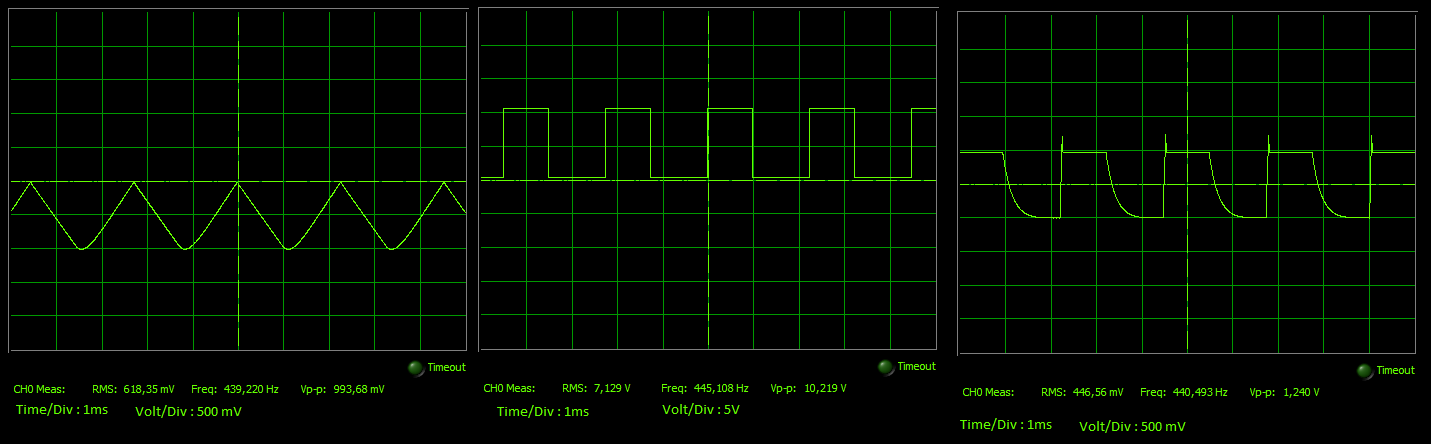
\includegraphics[width=0.8\textwidth]{img/vco_real_out.png}
	\caption{Sortie des différens blocs. De gauche à droite. Sortie de l'integrator, sortie du trigger et sortie de l'integrator controller}
	\label{fig:out_vco_real}
\end{figure}
La figure \ref{fig:out_vco_real}montre les même signaux que la figure \ref{fig:out_vco_th} mais effectuée sur le circuit réel pour une tension d'entrée de 500 mV. Les différences entre les deux sont très faibles mise à part la sortie du bloc integrator controller qui en descente ne passe pas directement de on à off mais le fait progressivement. Cela provient du switch qui ne s'ouvre pas d'un coup.

La figure \ref{fig:theory_vs_mesure} montre que la réalité est la théorie sont très proche. Les différences observées sont dues à des imprécisions des valeurs des résistances et des capacités. Cela provient aussi du switch qui contrairement au modèle utilisé dans les simulations et les calculs possède une légère courbe d'hystérèse.
\begin{figure}
	\centering
	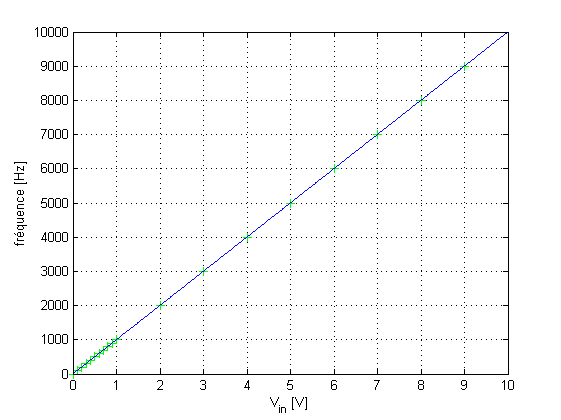
\includegraphics[scale=0.7]{img/vco_vs_reality.png}
	\caption{ Théroie Vs. mesures}
	\label{fig:theory_vs_mesure}
\end{figure}
\end{document}